\title{\huge Distribuerede Systemer \\
       \small Afleveringsopgave - 2 }
\author{Hold: DA4; Gruppe: 2\\ \\
        \href{mailto:skeen@cs.au.dk}{Emil Madsen - 20105376}\\
        \href{mailto:emray@cs.au.dk}{Rasmus - 20105109}\\
        \href{mailto:sverre@cs.au.dk}{Sverre - 20083549}
       }
\date{\today}

\maketitle

\hrule

\section*{Overblik}

Vi har implementeret et objectorienteret design af en bank p� en Java server.

\begin{figure}[htb]
\center
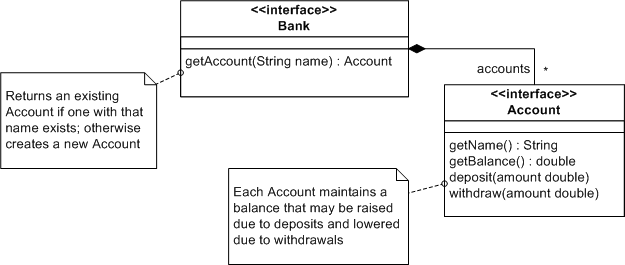
\includegraphics[width=\textwidth]{bankUML}
\caption{UML for Simpel bankapplikation}
\end{figure}

Man kan kommunikere med banken vha. vores implementation af RPC\footnote{RPC:
Remote Procedure Call}.

Denne rapport pr�ver at d�kke det f�lgende:
\begin{itemize*}
\item Vores protokol til at kommunikere med serveren (encoding format)
\item Vores testmetode og data
\item Hvordan serveren h�ndterer det at overs�tte klientkommunikationen til kald af Java objekter.
\end{itemize*}
Som i den tidligere aflevering er der vedlagt et Ant build script. 

K�r blot 'ant server' for at komme igang og se evt. Appendix A for yderligere
inspiration i form af et trace af en testsession.

\newpage
\section*{Protokol (Encoding Format)}
 Vi laver et \http \;(\proc{get}-)request, hvor Request-URI'en skal v�re formatteret s�ledes:

\begin{verbatim}
/<Class>/<Object>/<Method>?<Param_0>=<value_0>& ... &<Param_i>=<arg_i>
\end{verbatim}
 
\verb+<Class>+ betegner den relevante klasse, alts� f.eks. \verb+Bank+ eller \verb+Account+.

\verb+<Object>+ lader os kende forskel p� forskellige instanser af klasser, som
serveren holder.
Der kan f.eks. v�re flere Accounts.
Bank-klassen har altid 1 som v�rdi for objektet.

\verb+<Method>+ er den metode man gerne vil kalde.
Navnene er som beskrevet i UML'en.
 
\verb+<Param_0>=<value_0>+ er parameter til metoden.
Hvilken skal have samme navn som beskrevet af metoden selv i UML'en.
Der kan v�re vilk�rligt mange parametre, selvom ingen af bank eller account metoderne bruger mere end en.
\verb+param_0+ er s� navnet p� parameteren imf. UML'en, og \verb+value+ er v�rdien af parameteren.

Vi har tilladt os at afvige fra UML'en p� et punkt: 
Alle metoderne tager kun strenge som argumenter. 
Hvis det er en double, der skal bruges, skal metoden alts� konvertere strengen
f�rst.

\section*{Testmetode og data}
 For at teste koden kan man starte serveren via WebServer klassen og sende
kommandoer til den med en web browser.

Data opretholdes kun i serverens levetid.

En test kan best� af eksempelvis f�lgende Requests-URI\footnote{De listede strenge skal s�ttes efter \proc{url}'en, hvis testet i en browser, der har peget sig ind p� serveren.}:
\begin{verbatim}
   /Bank/1/getAccount?name=derp
   /Account/derp/getBalance?
   
   /Account/derp/deposit?amount=5
   /Account/derp/getBalance
   
   /Account/derp/withdraw?amount=10
   /Account/derp/getBalance
   
   /Account/derp/getName
\end{verbatim}
   
Hvis man for eksempel vil inds�tte 500 til Jimmy's konto, kalder man
\verb+getAccount(jimmy)+ ved
\begin{verbatim}/Bank/1/getAccount?name=jimmy\end{verbatim} og
bruger resultatet som \verb+<Object>+ til \verb+deposit(500)+, hvilket s�ledes
bliver:
\begin{verbatim}/Account/<Object>/deposit?amount=500\end{verbatim}

I tilf�lde af at en konto bliver efterspurgt via \verb+getAccount+, men ikke eksisterer, vil en konto p� det navn blive oprettet med et kontobel�b p� 0.0.

\section*{Serverens konvertering af Request-URI'en }
 Serveren modtager \proc{get}-requests eller \proc{post}-requests, hvor
Request-URI'en overholder protokollen\footnote{Bem�rk: Vi har prioriteret
sanitizing af indkommende requests lavt indtil videre. V�r varlig.}. 

Serveren deler Request-URI'en op i de af protokollen specificerede dele:
\id{class}, \id{object}, \id{method} og derudover en r�kke parametre og
v�rdier (\id{arguments}).

Derefter s�ger den efter det Java klasse-objekt, der matcher
\id{class}\footnote{Dette foreg�r ved opslag i classloaderen (register over
klasser i den lokale JVM)}, 

Den fundne \texttt{klasse} erkl�rer en r�kke metoder, som ledes igennem for at
finde den \texttt{metode} der matcher \id{method}.

Serveren holder et map, hvor \id{object} er n�gle til et Java \texttt{objekt}.
Dette map initialiseres sammen med serveren og vedligeholdes ved tilf�jelse af
flere kontoer/banker (eller fjernelse).

Alts� finder serveren det \texttt{objekt}, der matcher med \id{object} i
mappet, og kalder \texttt{metoden} p� \texttt{objektet} med \id{argumenterne}. 

\id{Resultatet} returneres til klienten.

\begin{figure}[htbp]
\center
\begin{adjustbox}{max size={.8\textwidth}{.6\textheight}}
\tikzstyle{decision} = [diamond, draw, fill=blue!20,
    text width=4.8em, text badly centered, node distance=2.7cm, inner sep=0pt]
\tikzstyle{block} = [rectangle, draw, fill=blue!20,
    text width=5em, text centered, rounded corners, minimum height=4em]
\tikzstyle{blockwide} = [rectangle, draw, fill=blue!20,
    text width=10em, text centered, node distance=1.4cm, rounded corners, minimum height=2em]
\tikzstyle{line} = [draw, very thick, color=black!50, -latex']
\tikzstyle{cloud} = [draw, ellipse,fill=red!20, node distance=3.5cm,
    minimum height=2.4em]
\tikzstyle{block2} = [rectangle, draw, fill=red!20,
    text width=5em, text centered, rounded corners, minimum height=4em]
\tikzstyle{case} = [near start, color=black]

\begin{tikzpicture}[scale=2, node distance = 3.5cm, auto]

    % Place nodes
    \node [cloud] (init) 
            {Server Method Dispatch};
    \node [blockwide, below of=init] (intro)
            {Tokenize URI-Request };
    \node [decision, below of=intro] (gotClass) 
            {Does the JVM recognize the \id{class}?};
    \node [cloud, below left of=gotClass] (error) 
            {error};
    \node [block, right of=gotClass] (yClass) 
            {\texttt{Class} variable stored};
    \node [decision, below of=yClass] (gotMethod) 
            {Do the \texttt{Class} declare the \id{method}?};
    \node [block, right of=gotMethod] (yMethod) 
            {\texttt{Method} variable stored};
    \node [decision, below of=yMethod] (gotMapping) 
            {Is the \texttt{class} mapped by \id{object}?};
    \node [block, below of=gotMapping] (yMapping) 
            {\texttt{Object} retrieved from map and stored};
    \node [block, left of=yMapping] (parse) 
            {Parse \id{arguments}};
    \node [block, left of=parse] (invoke) 
            {Invoke \texttt{Method} on \texttt{Object} with \texttt{Arguments}};
    \node [block2, left of=invoke] (fin) 
            {Return \id{result} from the method call};

    % Draw edges
    \path [line] (init) -- (intro);
    \path [line] (intro) -- (gotClass);
    \path [line] (gotClass) -- node [case] {No} (error);
    \path [line] (gotClass) -- node [case] {Yes} (yClass);
    \path [line] (yClass) -- (gotMethod);
    \path [line] (gotMethod) -- node [case] {No} (error);
    \path [line] (gotMethod) -- node [case] {Yes} (yMethod);
    \path [line] (yMethod) -- (gotMapping);
    \path [line] (gotMapping) -| node [case] {No} (error);
    \path [line] (gotMapping) -- node [case] {Yes} (yMapping);
    \path [line] (yMapping) -- (parse);
    \path [line] (parse) -- (invoke);
    \path [line] (invoke) -- (fin);
\end{tikzpicture}

\end{adjustbox}
\caption{Flow diagram, der viser hvordan serveren konverterer URI-requesten til
et metodekald.}
\end{figure}


\newpage
\section*{Appendix A \\
    \small Dette er et trace af en af vores test-sessioner: 
}
\VerbatimInput[frame=leftline,numbers=left,numbersep=3pt,fontsize=\footnotesize]{trace-run.txt}
